\documentclass[a4paper,12pt]{article}
    \usepackage[utf8]{inputenc}
    \usepackage[T1]{fontenc}
    \usepackage[english]{babel}
    \usepackage{graphicx}
    \usepackage{geometry}
    \geometry{a4paper,
                 tmargin = 35mm, 
                 lmargin = 25mm,
                 rmargin = 30mm,
                 bmargin = 30mm}
    \usepackage{mathtools}
    \usepackage{amsmath} % or simply amstext
	\newcommand{\angstrom}{\textup{\AA}}
    \usepackage{color}
    \usepackage{setspace}
    \usepackage{enumitem}
    \usepackage{amsmath,amssymb}
    \usepackage{float}
	\usepackage{listings}
	\usepackage{hyperref}
    
    \usepackage{indentfirst}
	\usepackage{subfig}
	    
    \renewcommand\thesection{\Roman{section}.}
    \renewcommand\thesubsection{\thesection\arabic{subsection}}
    \renewcommand\thesubsubsection{}
    
\begin{document}

\linespread{1.2}

\begin{titlepage}

	\centering
	{\scshape\LARGE ELTE Faculty of Science\par}
	\vspace{2cm}
	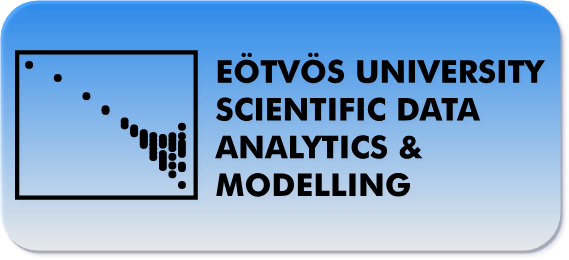
\includegraphics[width=0.66\textwidth]{./dslogo.png}
	\par\vspace{4cm}
	{\scshape\Large Twitter localization\par}
	\vspace{.5cm}
	{\large\itshape Alex Olar \par}
	\vfill
	{\large 2018 \par}

\end{titlepage}

\onehalfspacing

\begin{abstract}
	\par During the years the university has built a database 
	using Twitter's public API and collected more than 3 TB of
	data to analyze. I got access to this dataset and attempted
	to predict the location of users based on their followers'
	location.
	\par The problem itself is not a machine learning problem but
	an analytical approach and making assumptions about the behavior
	of users. Therefore I put an emphasis on visualization since the
	most crucial thing one does before any algorithmic solution
	is to analyze the visualized dataset.
\end{abstract}

\tableofcontents

\newpage

\section{The dataset}

\par I was provided with an undirected, full graph with bidirectional
data of followers. Meaning that the dataset I was given included all the
users and their followers who they followed as well. 

\vspace{.2cm}

\par \textit{Assumption I.:} This is already an assumption that the users
themselves follow many celebrities, stars, artists whom are not following 
them, therefore their location is not relevant.

\vspace{.2cm}

\par The graph was stored in SQL with and the following properties were
present: \textit{userId}, \textit{followerId}, \textit{userLon}, \textit{userLat},
\textit{followerLon}, \textit{followerLan}, \textit{dist}.

\vspace{.2cm}

\par I have not used the distance metric at all because I did not need in
in my process of finding the best location to predict. However, this kind
of dumped data layout was not very useful for my data exploration since I
didn't exactly have the followers' list of a user and therefore I could not
say anything about their location.

\vspace{.2cm}

\par Firstly I built a table with acquiring all the \textit{userId}s and 
their geographical locations. This is called later on \textit{Twitter\_User}. 
I acquired this by running the following query:

\vspace{.2cm}

\lstset{language=SQL}
\lstset{frame=lines}
\lstset{caption={Building the user table}}
\lstset{basicstyle=\footnotesize}
\begin{lstlisting}
  INSERT INTO Twitter_User (ID, lon, lat)
      SELECT DISTINCT id as ID, lon, lat
      FROM follower_graph;
\end{lstlisting}

\vspace{.2cm}

\par On this table I set up \textit{ID} as \textit{PRIMARY KEY} since
the indexing of the data, which was not present on the follower graph table
made the querying process way faster. I copied that table as well and set
the \textit{(userId, followerId)} pair as \textit{PRIMARY KEY} and did a join
on the data tables in order to acquire all the data from the DB in order.
This process resulted in \textbf{$\approx$ 94 million)} rows which is approximately
5 GBs of data. The \textit{Twitter\_User} table contained \textbf{$\approx$ 3.2 million}
users.

\vspace{.2cm}

\lstset{language=SQL}
\lstset{frame=lines}
\lstset{caption={Building the user table}}
\lstset{basicstyle=\footnotesize}
\begin{lstlisting}
  SELECT follower.fid, follower.flon,
    follower.flat, follower.dist,
    twitter_user.lon, twitter_user.lat,
    twitter_user.ID
  FROM alex..Twitter_User as twitter_user
  INNER JOIN alex..follower_graph as follower
    ON twitter_user.ID = follower.id
  ORDER BY twitter_user.ID
\end{lstlisting}

\par After acquiring the data it was obvious how to proceed. I created
a dictionary where the keys were the user ids and one record contained all 
the follower ids and locations of the followers and as many types the user's
location as well, this part was sadly not optimized.

\vspace{.2cm}

\par Having gathered all the necessary information about the users I
could move on the the general algorithm of localization.

\section{The essence of localization}

\par Using the locations of the user's followers I wanted to select the largest
group of closest followers and get the mean of their locations. The problem and 
the solution is well described but the implementation is not that straightforward
since the locations are provided as geographical coordinates, so not only is clustering not
trivial on the surface of the globe but also it is somewhat complicated to get 
the mean location of the users.

\vspace{.2cm}

\par Since the number of clusters could not be estimated beforehand and I wanted to
select the most densely populated neighbor cluster I used \textbf{DBSCAN} \cite{dbscan} clustering
which is density based and can relatively well cluster this type of data.
It was also a huge advantage that the \textit{sklearn} \cite{sklearn} package included the 
\textit{Haversine} metric.

\vspace{.2cm}

\par The \textit{Haversince formula} determines the great-circle distance 
between two points on a sphere given their longitudes and latitudes \cite{wiki_haversine}.
The haversine function of an angle $\vartheta$ is given in the form:

\vspace{.2cm}

\begin{equation*}
	hav(\vartheta) = sin^{2}\Big(\frac{\vartheta}{2}\Big) = \frac{1-cos(\vartheta)}{2}
\end{equation*}

\vspace{.2cm}

\par Where $\vartheta$ is the angle - longitude or latitude - of a point. The central angle
$\Theta$ is defined as the fraction of the distance of the points over the radius \textbf{R}
of the sphere which is \textit{6371 km} this case. The Haversine formula is described then as:

\vspace{.2cm}

\begin{equation*}
	hav(\Theta) = hav(\varphi_{2} - \varphi_{1}) + cos(\varphi_{1})cos(\varphi_{2})hav(\lambda_{2} - \lambda_{1})
\end{equation*}

\vspace{.2cm}

\par The distance can be derived from this formula. \textit{DBSCAN} takes a few more
arguments such as minimal distance to cluster on which was set to $\frac{5.}{6371.}$
( $\equiv$ 5 km ) and the minimum samples in a cluster was set to 5. The longitudes and latitudes
were converted to radians and the clustering was done.

\vspace{.2cm}

\par The algorithm generates outliers as well and sometimes there are no clusters at all. In all
those cases I just converted the geographical coordinates to cartesian coordinates, averaged them
and converted back to geolocations. For proper conversion I used the \textit{astropy} package
which provided an implementation of conversion.

\vspace{.2cm}

\par On the other hand, when the clustering was done properly I selected the largest cluster of
the followers of a user and averaged their locations as the above described manner.

\vspace{.2cm}

\par Finally I created a dataset with the predicted and actual locations of the users
and generated 50 filtered dataset based on maximum distance between the predicted and actual 
locations. With this method I acquired some kind of accuracy metric:

\vspace{.2cm}

\begin{figure}[H]
	\centering
	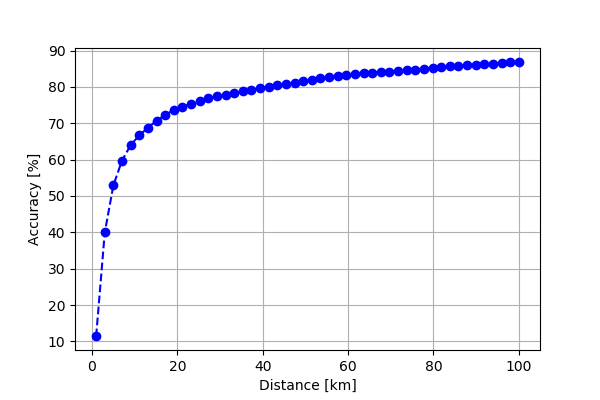
\includegraphics[width=0.7\textwidth]{./accuracy-distance.png}
	\caption{Accuracy on maximum distance allowed}
\end{figure}

\vspace{.2cm}

\par The accuracy of prediction is really good for 100 km, although, it is not that bad for
1 km either since it acquired more than 10 \% precision which I assume could be much higher
making the prediction only in a city f.g. \textit{New York}. Lowering the scale from 0 to 1 km:

\vspace{.2cm}

\begin{figure}[H]
	\centering
	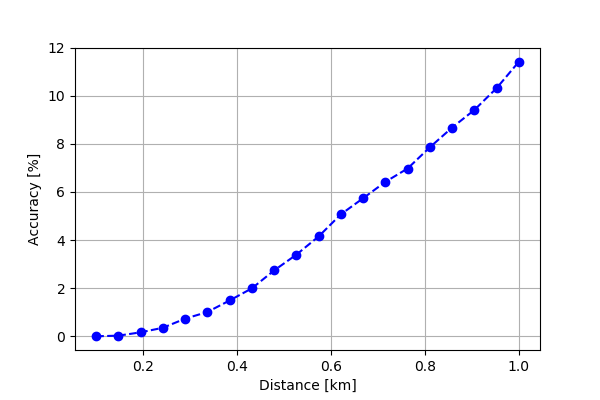
\includegraphics[width=0.7\textwidth]{./fine-accuracy-distance.png}
	\caption{Accuracy on maximum distance allowed - finer scale}
\end{figure}

\par There is no point in raising the maximum distance more therefore I am
not calculating the accuracy in that case. The accuracy was simply acquired by
taking the maximum number of predicted points and dividing by it on the filtered points.
Unfortunately the distance calculation in this period was not based on the Haversine metric but
on basic cartesian distance, although, it is not completely inaccurate in this 0 - 100 km scale.

\section{The visualization}

\par The visualization tool is reachable at \url{https://twitter-localization.herokuapp.com}. It consists 
of a data providing backend, hosted on Heroku as well. The backend has saved \textit{csv}
files on different maximum distances and each of those is fed to the Angular 
frontend using Leaflet.js \cite{leaflet} as visualization tool. This package provides zoomable, and 
scaleable maps in JavaScript for the web. Little Twitter icons show the predicted
and actual locations of users (red and blue icons) and they are connected by a straight blue
line.

\vspace{.2cm}

\par The tool provides a slider with which it is possible to change the maximum
distance allowed and shows the accuracy metric and displayed number of points on the
map. I include screen shots but it can be tested on the fly during the lecture.

\vspace{.2cm}

\begin{figure}[H]
	\centering
	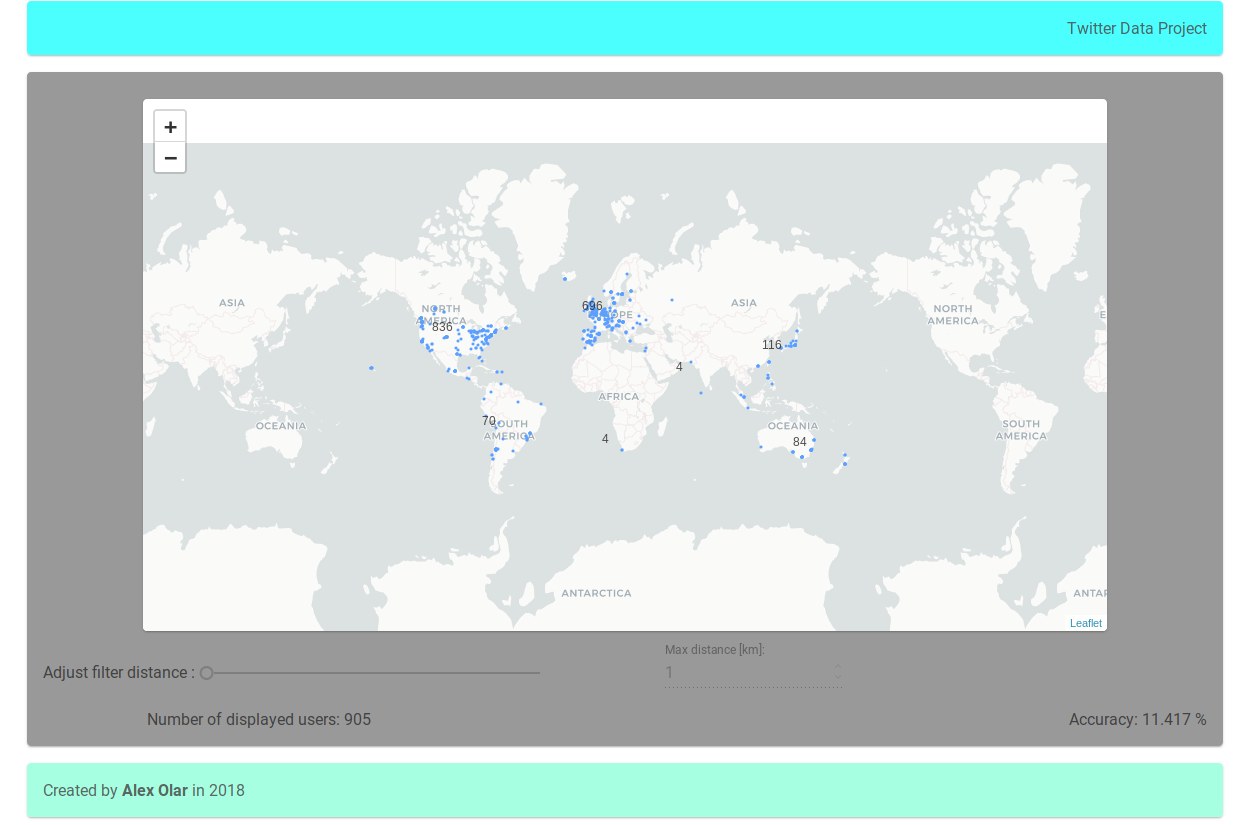
\includegraphics[width=0.6\textwidth, height=0.35\textwidth]{./twitter1.png}
	\caption{Default value - full}
\end{figure}

\vspace{.2cm}

\begin{figure}[H]
	\centering
	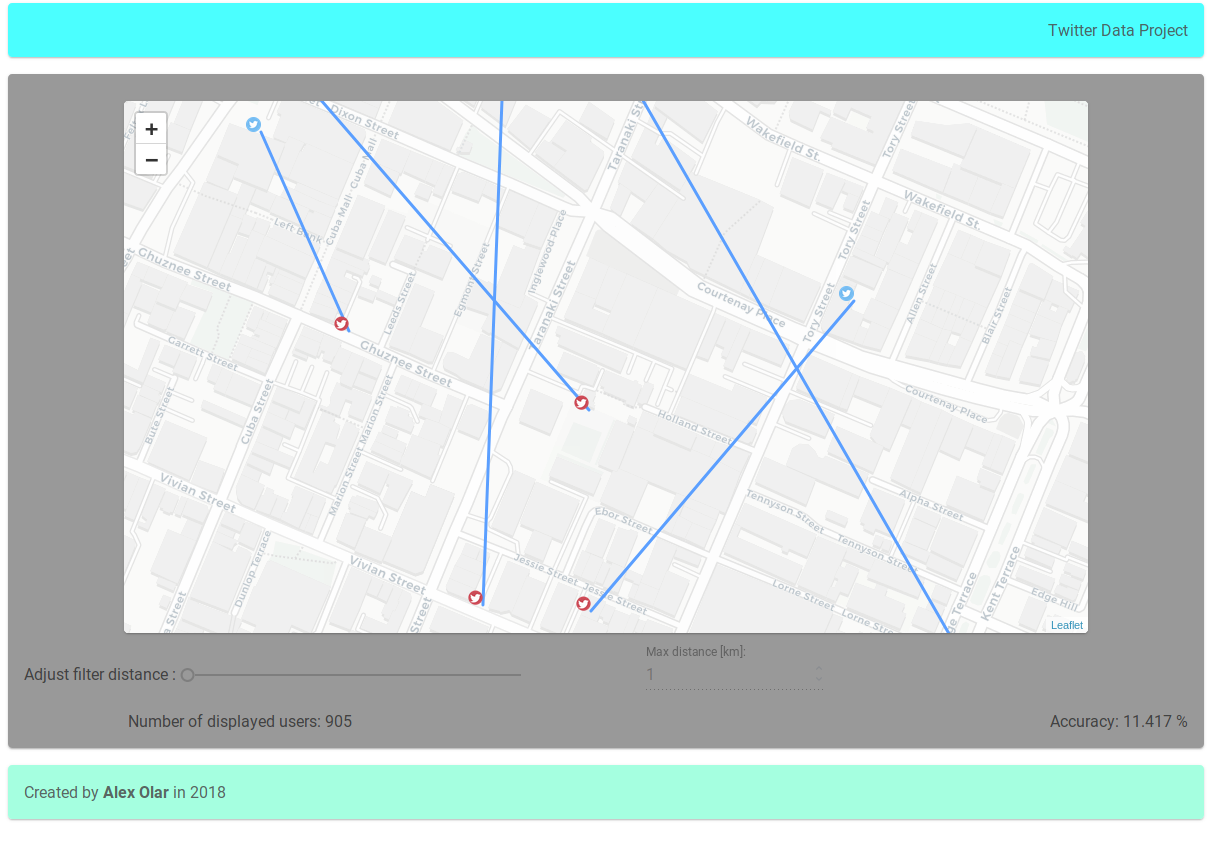
\includegraphics[width=0.6\textwidth, height=0.35\textwidth]{./twitter2.png}
	\caption{Default value - zoomed}
\end{figure}

\vspace{.2cm}

\begin{figure}[H]
	\centering
	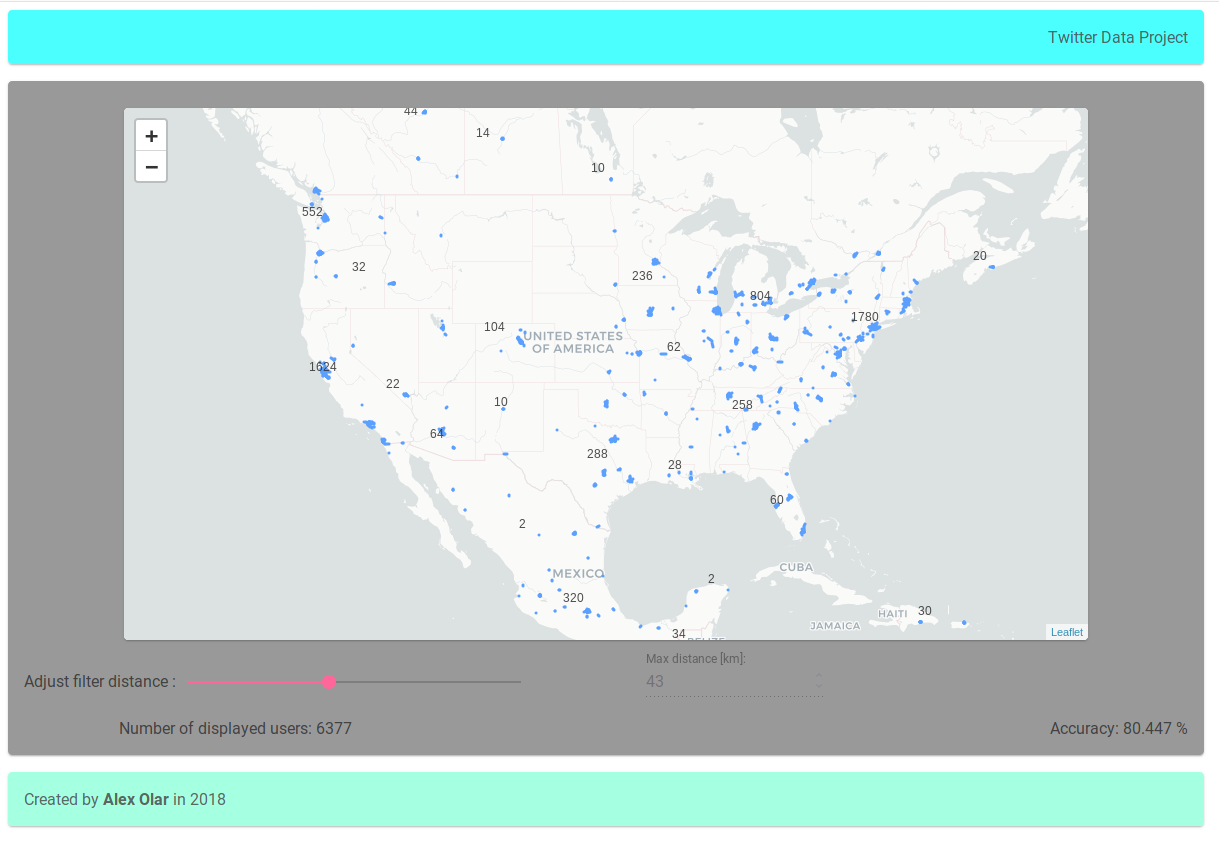
\includegraphics[width=0.6\textwidth, height=0.35\textwidth]{./twitter3.png}
	\caption{Changed distance - zoomed - USA}
\end{figure}

\section{Issues}

\par During the week of submission I was only able to connect to the server once.
Since I did not save the 5GB of data but waited that 2 minutes each and every time
to query it I could not process all the data. My algorithm does not even scale very
well, therefore I am not sure if it were possible at all. What I had is around 10 000
users with predicted and actual locations saved with distance in \textit{csv} two
weeks ago. However, I consider the project finished since as the data processed is
most probably has the same statistics as the rest of it and I processed around 
2 \% of the total dataset.

\section{Overview}

\par Therefore I completed all the tasks required to finish this project. I was 
not sure whether the visualization tool is enough progress or not. It is not that
straightforward to do these things as it seems and there are some very nitpicky
moments during the process.

\vspace{.2cm}

\par My work can be found on GitHub \cite{qbeer} and on my Heroku \cite{deployed_app}.

\newpage
\bibliographystyle{plain}
\bibliography{references}

\end{document}